\documentclass[a4paper, 12pt, notitlepage]{report}

\usepackage[utf8]{inputenc}
\usepackage[T5]{fontenc}
\usepackage{tgheros}

\usepackage{array}
\usepackage{amsmath}
\usepackage{amssymb}
\usepackage{amsthm}
\usepackage{biblatex}
\usepackage{blindtext}
\usepackage{enumerate}
\usepackage{fancyhdr}
\usepackage{float}
\usepackage{geometry}
\usepackage{graphicx}
\usepackage{lipsum}
\usepackage{listings}
\usepackage{multicol}
\usepackage{tikz}
\usepackage{xcolor}
\usepackage{tabulary}
\usepackage[unicode]{hyperref}

% UPDATED: Changed from sample.bib to references.bib
\addbibresource{references.bib}
\graphicspath{{sections/images/}{images/}}

\renewcommand{\familydefault}{\rmdefault}
\renewcommand{\figurename}{Figure}

\geometry{
	a4paper,
	left=20mm,
	right=20mm,
	bindingoffset=0mm,
	top=30mm,
	bottom=25mm,
	headheight=30pt
}

\linespread{1.3}

\newcommand{\linia}{\rule{\linewidth}{0.5pt}}

\makeatletter
\renewcommand{\maketitle}{
\begin{center}
	\vspace{2ex}
	{ \huge \textsc{\@title} }
	\vspace{1ex}
	\\ \linia\\ \@author \hfill \@date
	\vspace{4ex}
\end{center}
}
\makeatother

\setlength{\headheight}{30pt}
\fancyhead{}

\fancyhead[L]{
    \begin{tabular}{rl}
        \begin{picture}(15,10)(0,0)
            \put(0,-8){
                
\includegraphics[width=8mm, height=8mm]{vgu_logo.png}
            }
        \end{picture}
        &
        \begin{tabular}{l}
            \textbf{\textsf{Vietnamese-German University}}\\
            \textbf{\textsf{Department of Computer Science}}
        \end{tabular}
    \end{tabular}
}

\fancyhead[R]{}

\fancyfoot{}
\fancyfoot[L]{\ttfamily Customer Segmentation Analysis}
\fancyfoot[R]{\ttfamily Page \thepage}

\fancypagestyle{plain}{
    \fancyhead{}
    \fancyfoot{}
    \fancyfoot[L]{\ttfamily Customer Segmentation Analysis}
    \fancyfoot[R]{\ttfamily Page \thepage}
}

\renewcommand{\headrulewidth}{0.2pt}
\renewcommand{\footrulewidth}{0.2pt}


% Define custom colors for SQL styling
\definecolor{codegreen}{rgb}{0,0.6,0}
\definecolor{codegray}{rgb}{0.5,0.5,0.5}
\definecolor{codepurple}{rgb}{0.58,0,0.82}
\definecolor{backcolour}{rgb}{0.95,0.95,0.92}

\lstset{
    language=SQL,
    backgroundcolor=\color{backcolour},   
    commentstyle=\color{codegreen},
    keywordstyle=\color{blue},
    numberstyle=\tiny\color{codegray},
    stringstyle=\color{codepurple},
    basicstyle=\ttfamily\small,
    breakatwhitespace=false,         
    breaklines=true,                 
    captionpos=b,                    
    keepspaces=true,                 
    numbers=left,                    
    numbersep=5pt,                  
    showspaces=false,                
    showstringspaces=false,
    showtabs=false,                  
    tabsize=4
}

\begin{document}
\hypersetup{pageanchor=false}
\begin{titlepage}
\begin{center}
    VIETNAMESE - GERMAN UNIVERSITY \\ DEPARTMENT OF COMPUTER SCIENCE
\end{center}

\vspace{1cm}

\begin{center}
    
\includegraphics[width=3cm]{vgu_logo.png}
\end{center}

\vspace{2cm}

\begin{center}
    \begin{tabular}{c}
        \textbf{\Large Customer Segmentation Analysis REPORT} \\
        \\
        \\
        \textbf{\Large Customer and Segmentation Data Analytics}                      \\
        \vspace{1cm}
    \end{tabular}
\end{center}

\vspace{2cm}

\begin{center}
    \begin{tabular}{rl}
        \hspace{5.1cm} \textit{Instructor:} & Phan Trọng Nhân, PhD             \\
        \\
        \textit{Student 1:} & Dương Quý Trang - 10423110         \\
        \textit{Student 2:} & Nguyễn Hà Khải - 10423053      \\
        \textit{Student 3:} & Nguyễn Quang Ngọc Trác - 10423109 \\
        \textit{Student 4:} & Tô Huỳnh Phúc - 10423093       \\
        \textit{Student 5:} & Nguyễn Hữu Triển - 17813     \\
    \end{tabular}
\end{center}

\vspace{2cm}
\begin{center}
    { \footnotesize BÌNH DƯƠNG CITY, 10/2026 }
\end{center}
\end{titlepage}
\hypersetup{pageanchor=true}

\pagenumbering{roman}
\pagestyle{fancy}



\newpage
\listoftables
\listoffigures

\newpage
\renewcommand{\contentsname}{Contents}
\vspace{1cm}
\tableofcontents

\newpage
\pagenumbering{arabic}

% ==========================================
% Main Content (Decoupled Sections)
% ==========================================
\chapter{Introduction}
\label{chap:introduction}

\section{Project Context and Data Source}
Customer purchasing behaviour is an important input to retail decisions, yet transaction tables alone do not readily
show which customers buy repeatedly, which customers generate high value, or which customer groups require different
marketing approaches. CompanyX is the retail dataset used in this project. Its transactional schema records customers,
sales orders, order details, products, and associated customer demographics. The available sales history begins in May
2011 and ends in June 2014.

The project deliberately focuses on \emph{customer-centric analysis}, rather than general sales reporting. In
particular, the team uses Recency, Frequency, and Monetary (RFM) behaviour to describe customers, K-Means to discover
five interpretable groups, and a dimensional data warehouse to make these results available for analysis. The warehouse
also stores slowly changing customer attributes and monthly historical observations. Its automated ETL pipeline makes
the latest customer profiles and purchase-triggered segmentation results available at one-minute intervals.

\section{Business Problem}
The practical question is not simply how much CompanyX sold, but \emph{which customers contributed that value and how
  their purchasing patterns changed}. Four issues motivated the solution:
\begin{itemize}
  \item \textbf{Repeat purchasing and retention.} Single-order buyers and customers who do not return represent different opportunities from loyal repeat customers. An appropriate intervention requires a view of their purchase frequency and time since their last order.
  \item \textbf{Uneven customer value.} Customers differ considerably in their spending. Treating all customers identically can hide high-value accounts and lead to inefficient campaign allocation.
  \item \textbf{Cross-selling opportunities.} Understanding a customer's value and engagement stage can help marketers decide when to recommend accessories, maintenance products, or complementary items. RFM identifies target groups; verifying product-specific cross-selling gaps would require separate product-level analysis.
  \item \textbf{Fragmented historical and operational views.} A record updated when a purchase occurs answers a different question from a month-end view of the entire customer population. Both are needed to distinguish purchase-time behaviour from longer-term inactivity and segment migration.
\end{itemize}

The Power BI dashboard provides key indicators such as repeat-customer rate, customer inactivity, average purchase
frequency, and spending patterns. Together, these metrics offer an overview of customer purchasing behavior and
engagement, helping decision-makers identify potential retention issues, understand customer value, and develop
appropriate marketing strategies.

\section{Objectives and Deliverables}

The primary objective of this project is to develop a customer segmentation and business intelligence system that helps
CompanyX better understand customer purchasing behaviour and support data-driven decision-making. The project focuses
on two main goals:

\begin{enumerate}
  \item \textbf{Customer Segmentation:}
        Analyse customer purchasing patterns to identify distinct customer
        groups based on their behaviour and value. These insights can help
        the company better understand its customer base and develop more
        effective marketing, retention, and customer engagement strategies.

  \item \textbf{Automated Business Intelligence Pipeline:}
        Develop an integrated system that automatically collects, processes,
        and analyses customer data. The system aims to provide up-to-date
        customer information while maintaining historical records, allowing
        businesses to monitor changes in customer behaviour over time.
\end{enumerate}

To achieve these objectives, the project delivers an integrated solution consisting of a data warehouse, automated data
processing pipelines, machine learning-based customer segmentation, and interactive business intelligence dashboards.
Together, these components transform raw transactional data into meaningful insights that support business analysis and
decision-making.

\chapter{Theoretical Framework \& Industry Benchmark Case Studies}
\section{Context}

Write the project background, business context, and objectives here.

\subsection{Main issue}

Describe the key problem statements, current bottlenecks, and target solutions here.


\chapter{Datawarehose Design}
We propose our data warehouse design as below:

\begin{figure}[htbp]
    \centering % Căn giữa hình ảnh
    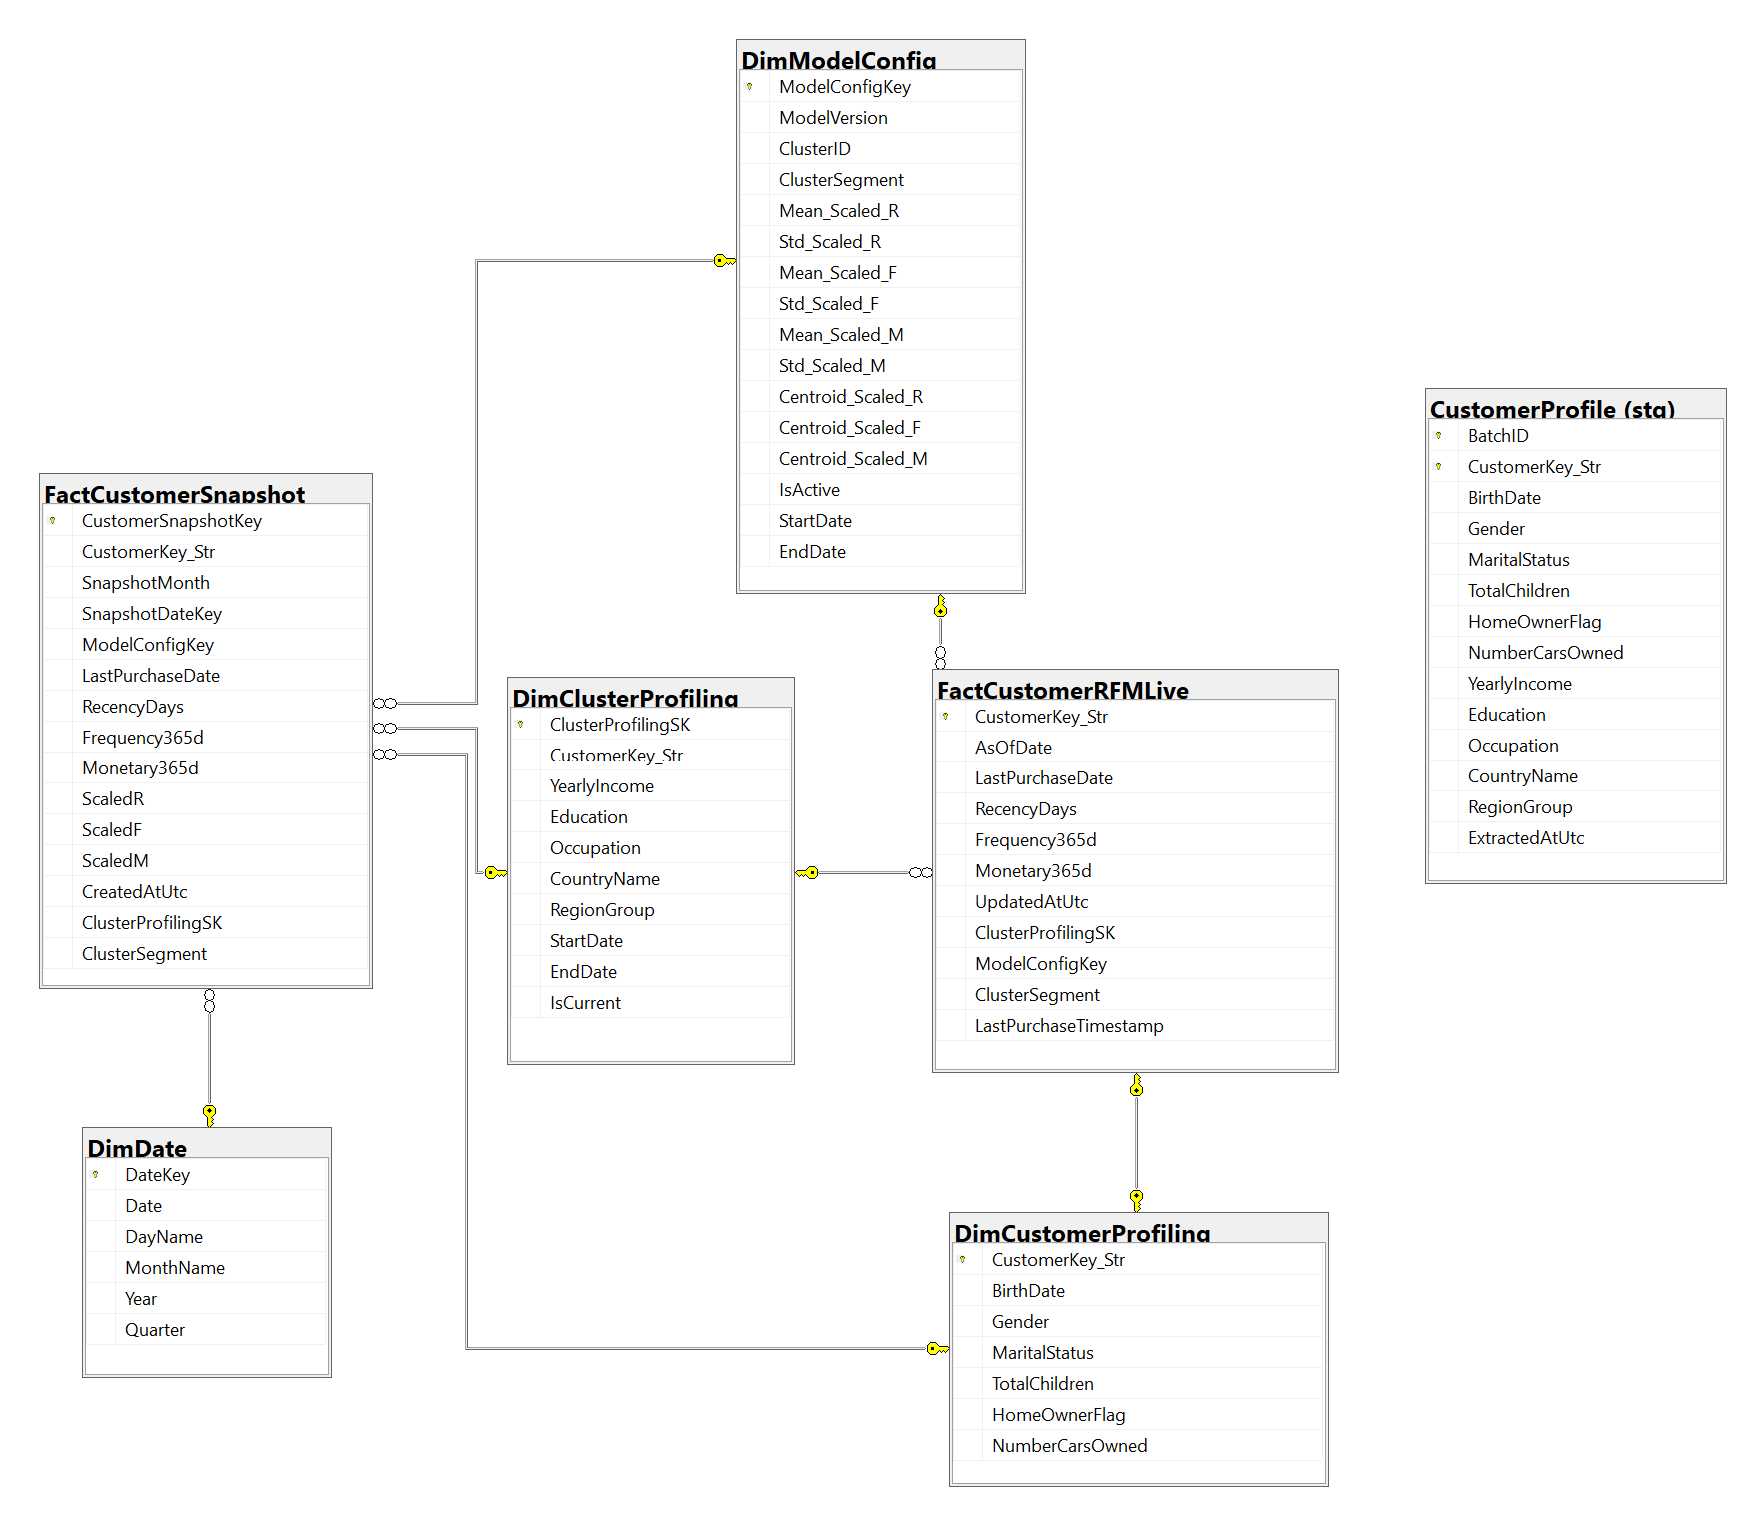
\includegraphics[width=0.8\textwidth]{DWHdesign.png}
    \caption{Đây là chú thích của hình ảnh.}
    \label{fig:DWH_design} % Nhãn để dùng cho lệnh tham chiếu \ref{}
\end{figure}

At a first glance, we can observe that the blueprint follows a hybrid constellation / star-galaxy schema which consists of two fact tables, namely FactCustomerSnapshot, FactCustomerRFMLive; four dimensions including \verb|DimModelConfig|, \verb|DimClusterProfiling|, \verb|DimDate|, \verb|DimCustomerProfiling|. 
\section{Context}

Write the project background, business context, and objectives here.

\subsection{Main issue}

Describe the key problem statements, current bottlenecks, and target solutions here.


\chapter{System Workflow}

\section{ETL Pipeline \& Data Flow}


\section{Dimension Layer \& Slowly Changing Dimension Strategy}

\subsection{DimCustomerProfiling}

\subsection{DimClusterProfiling}





% Chapter content only — insert with \input{customer_segmentation_chapter.tex}
\chapter{RFM Analysis and K-Means Clustering}\label{chap:ml}

\section{Motivation}

The CompanyX transactional database contains purchases from May 2011 through June 2014. However, raw sales records alone do not identify which customer groups require different business strategies. This chapter follows the team's implemented approach: summarize purchase behaviour using RFM, clean and transform the features, fit K-Means to customer snapshots, and translate the resulting numeric clusters into interpretable segment names. The trained configurations can then be reused by the operational scoring pipeline and historical snapshot process.

\subsection{RFM Variables}
Recency (R) is the number of days from an evaluation date to the customer's last purchase. Frequency (F) is the count of distinct sales orders within the trailing 365 days. Monetary (M) is the sum of order-line amounts within that same 365-day period. Recency may exceed 365 days for customers who have not purchased recently. The year-end training snapshots used by the project are 31 December 2011, 2012, and 2013; there is no 2014 trained model.

\section{Data Cleaning}

The raw data is first ingested from the FactCustomerSnapshot, and then processed through deduplication. After that, any
R, F, or M values are missing, the process stops and reports the number of affected rows to the ETL Team. Anomalies
values such as negative values are set to zero, since a purchase count or a monetary value can not be negative.

This subset of data serves a representative overview of customer purchases based on RFM analysis as mentioned above.

\begin{table}[htbp]
  \centering
  \small
  \begin{tabular}{rrrr}
    \hline
    \textbf{Customer} & \textbf{Recency} & \textbf{Frequency} & \textbf{Monetary} \\
    \hline
    11057             & 37               & 1                  & 3729.36           \\
    11058             & 22               & 1                  & 3756.99           \\
    11060             & 12               & 1                  & 3756.99           \\
    11061             & 18               & 1                  & 3729.36           \\
    11072             & 0                & 1                  & 3756.99           \\
    11238             & 84               & 1                  & 3756.99           \\
    11239             & 71               & 1                  & 3729.36           \\
    11240             & 32               & 1                  & 3756.99           \\
    11243             & 38               & 1                  & 3756.99           \\
    11244             & 47               & 1                  & 3756.99           \\
    11247             & 41               & 1                  & 3729.36           \\
    11250             & 14               & 1                  & 3756.99           \\
    11333             & 10               & 1                  & 3756.99           \\
    11334             & 27               & 1                  & 3756.99           \\
    11337             & 22               & 1                  & 3729.36           \\
    11591             & 79               & 1                  & 3953.99           \\
    11592             & 79               & 1                  & 3953.99           \\
    11593             & 69               & 1                  & 3953.99           \\
    11599             & 72               & 1                  & 3953.99           \\
    11601             & 71               & 1                  & 3953.99           \\
    11606             & 82               & 1                  & 3953.99           \\
    11607             & 71               & 1                  & 3953.99           \\
    \hline
  \end{tabular}
  \caption{Example RFM records before preprocessing.}\label{tab:rfm_sample}
\end{table}

\section{Log transformation}

Spending and purchase counts are usually right-skewed. Most customers spend a moderate amount, while only a small
number spend many times more. If raw values are used, these large values stretch the scale and the K-Means model spends
more effort unnecessarily separating a few high spenders (outliers) rather than grouping typical customers. By using
log transformation, the issue can be minimized.

For example, a customer who spends 3,000 and 300,000 differs by a factor of 100 in raw terms, but their log values
differ by only 4.6. We use log(1+x) in this case, written log1p because some customers have a value of zero, which
leads to log(0) undefined.

\begin{table}[htbp]
  \centering
  \small
  \begin{tabular}{rrrr}
    \hline
    \textbf{Customer} & \textbf{Recency} & \textbf{Frequency} & \textbf{Monetary} \\
    \hline
    11057             & 3.638            & 0.693              & 8.224             \\
    11058             & 3.135            & 0.693              & 8.232             \\
    11060             & 2.565            & 0.693              & 8.232             \\
    11061             & 2.944            & 0.693              & 8.224             \\
    11072             & 0.000            & 0.693              & 8.232             \\
    11238             & 4.443            & 0.693              & 8.232             \\
    11239             & 4.277            & 0.693              & 8.224             \\
    11240             & 3.497            & 0.693              & 8.232             \\
    11243             & 3.664            & 0.693              & 8.232             \\
    11244             & 3.871            & 0.693              & 8.232             \\
    11247             & 3.738            & 0.693              & 8.224             \\
    11250             & 2.708            & 0.693              & 8.232             \\
    11333             & 2.398            & 0.693              & 8.232             \\
    11334             & 3.332            & 0.693              & 8.232             \\
    11337             & 3.135            & 0.693              & 8.224             \\
    11591             & 4.382            & 0.693              & 8.283             \\
    11592             & 4.382            & 0.693              & 8.283             \\
    11593             & 4.248            & 0.693              & 8.283             \\
    11599             & 4.290            & 0.693              & 8.283             \\
    11601             & 4.277            & 0.693              & 8.283             \\
    11606             & 4.419            & 0.693              & 8.283             \\
    11607             & 4.277            & 0.693              & 8.283             \\
    \hline
  \end{tabular}
  \caption{Log-transformed sample RFM values.}
\end{table}

\section{Standardization}

Before importing data to run the K-Means Clustering model, it is essential to standardize the RFM values to ensure that
each metric contributes equally to the analysis, since Recency, Frequency, and Monetary values are measured on
different scales. K-Means relies heavily on distances (later will be shown), so a variable with a larger spread would
dominate the result.

StandardScaler solves this by subtracting the mean and dividing by the standard deviation of each variable, so that
each one has a mean of 0 and a standard deviation of 1. The mean and standard deviation are estimated from the training
data and stored, so that new customers are scaled in the same way.

\begin{table}[htbp]
  \centering
  \small
  \begin{tabular}{rrrr}
    \hline
    \textbf{Customer} & \textbf{Recency} & \textbf{Frequency} & \textbf{Monetary} \\
    \hline
    11057             & 0.109            & 0.000              & -0.875            \\
    11058             & -0.392           & 0.000              & -0.581            \\
    11060             & -0.962           & 0.000              & -0.581            \\
    11061             & -0.583           & 0.000              & -0.875            \\
    11072             & -3.522           & 0.000              & -0.581            \\
    11238             & 0.913            & 0.000              & -0.581            \\
    11239             & 0.747            & 0.000              & -0.875            \\
    11240             & -0.032           & 0.000              & -0.581            \\
    11243             & 0.135            & 0.000              & -0.581            \\
    11244             & 0.342            & 0.000              & -0.581            \\
    11247             & 0.209            & 0.000              & -0.875            \\
    11250             & -0.819           & 0.000              & -0.581            \\
    11333             & -1.128           & 0.000              & -0.581            \\
    11334             & -0.196           & 0.000              & -0.581            \\
    11337             & -0.392           & 0.000              & -0.875            \\
    11591             & 0.852            & 0.000              & 1.454             \\
    11592             & 0.852            & 0.000              & 1.454             \\
    11593             & 0.719            & 0.000              & 1.454             \\
    11599             & 0.761            & 0.000              & 1.454             \\
    11601             & 0.747            & 0.000              & 1.454             \\
    11606             & 0.889            & 0.000              & 1.454             \\
    11607             & 0.747            & 0.000              & 1.454             \\
    \hline
  \end{tabular}
  \caption{Standardized sample RFM values.}
\end{table}

\section{K-Means Clustering}

K-Means is an unsupervised algorithm that partitions observations into \(K\) clusters by iteratively assigning each point to the nearest centroid and updating centroid locations. The project fits scikit-learn \texttt{KMeans} with \(K=5\), \texttt{k-means++} initialization, \texttt{n\_init=10}, \texttt{max\_iter=300}, and \texttt{random\_state=42}.

For each data point in the dataset, calculate the Euclidean distance between the point and each centroid. Assign the
data point to the cluster with the closest centroid

\[ d(\mathbf{x},\mathbf{c}) = \sqrt{\sum_{j=1}^{3} (x_j-c_j)^2}. \]

Where:
\begin{itemize}
  \item $d(x, y)$: the distance between data point x and centroid y
  \item $y_i$: donates the value of the i-th attribute value of centroid y
  \item $x_i$: represents the i-th attribute of the data point x
  \item $i$ : refers to index of the attribute
  \item $n$ : indicates the total number of the attribute for each data point
\end{itemize}

Within-cluster sum of squares (WCSS), also called inertia, measures the total squared distance from observations to their assigned centroids:

\[ \mathrm{WCSS}=\sum_{k=1}^{K}\sum_{i\in S_k}\sum_{j=1}^{3}(x_{ij}-c_{kj})^2. \]

Where:
\begin{itemize}
  \item K: Total number of clusters.
  \item k: An index that refers to the current cluster, ranging from 1 to K.
  \item $S_k$: The set of data points assigned to cluster k.
  \item p: Number of features or dimensions in the dataset.
  \item j: An index that refers to the current feature or dimension, ranging from 1 to p.
  \item $x_{ij}$: The j-th feature value of the i-th data point.
  \item $\bar{x}_{kj}$: The mean value of the j-th feature in cluster k (i.e., the centroid's value).
  \item $(x_{ij} - \bar{x}_{kj})^2$: The squared Euclidean distance between the j-th feature of data point xi and the corresponding feature of the centroid of its cluster.
\end{itemize}

This WCSS can also be known as the Inertia, the lower means the tighter the data points are grouped. Another important
criteria, which is Silhouette, also needs to be considered. The silhouette score measures how well-separated and
cohesive clusters are in K-Means clustering. It evaluates each data point's fit relative to its own cluster versus
neighboring clusters.

Figures~\ref{fig:elbow_2013} and~\ref{fig:silhouette_2013} reproduce the diagnostic plots already saved with the project for the 31 December 2013 snapshot. Inertia decreases as \(K\) increases, while the silhouette metric measures separation between clusters. The silhouette score for \(K=5\) is approximately 0.518; \(K=2\) achieves a higher score (approximately 0.636) on this snapshot. Therefore five clusters were chosen as a \emph{business-interpretability trade-off}, supported by the elbow/silhouette diagnostics and the desire for distinct actionable customer profiles, not because five globally maximizes the silhouette score.

\begin{figure}[htbp]
  \centering
  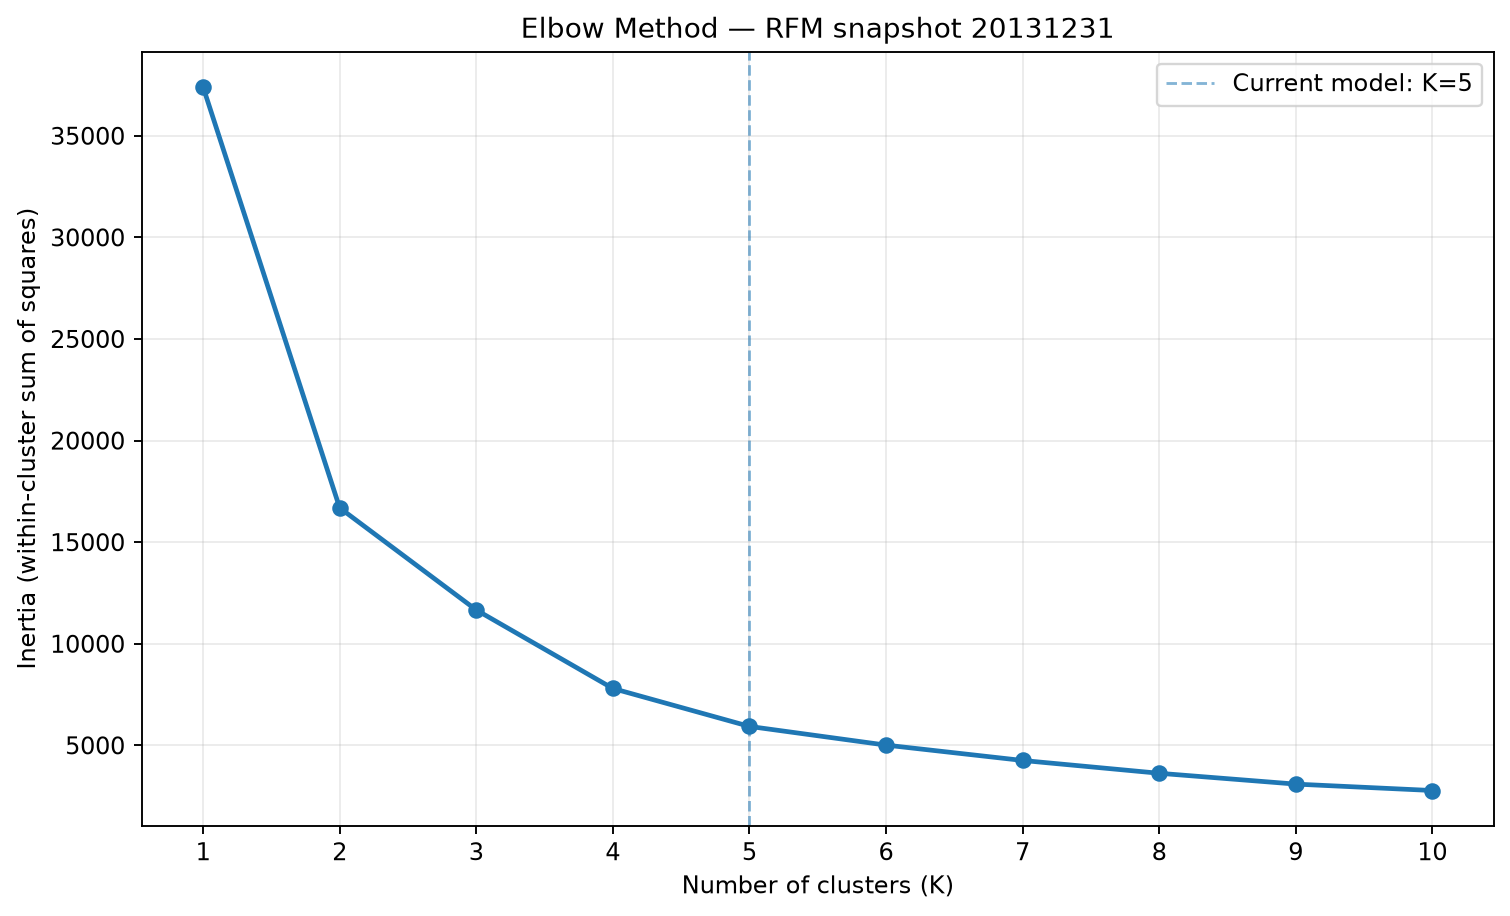
\includegraphics[width=0.94\textwidth]{elbow_20131231.png}
  \caption{Elbow plot for the 31 December 2013 RFM snapshot (existing project diagnostic).}
  \label{fig:elbow_2013}
\end{figure}
\begin{figure}[htbp]
  \centering
  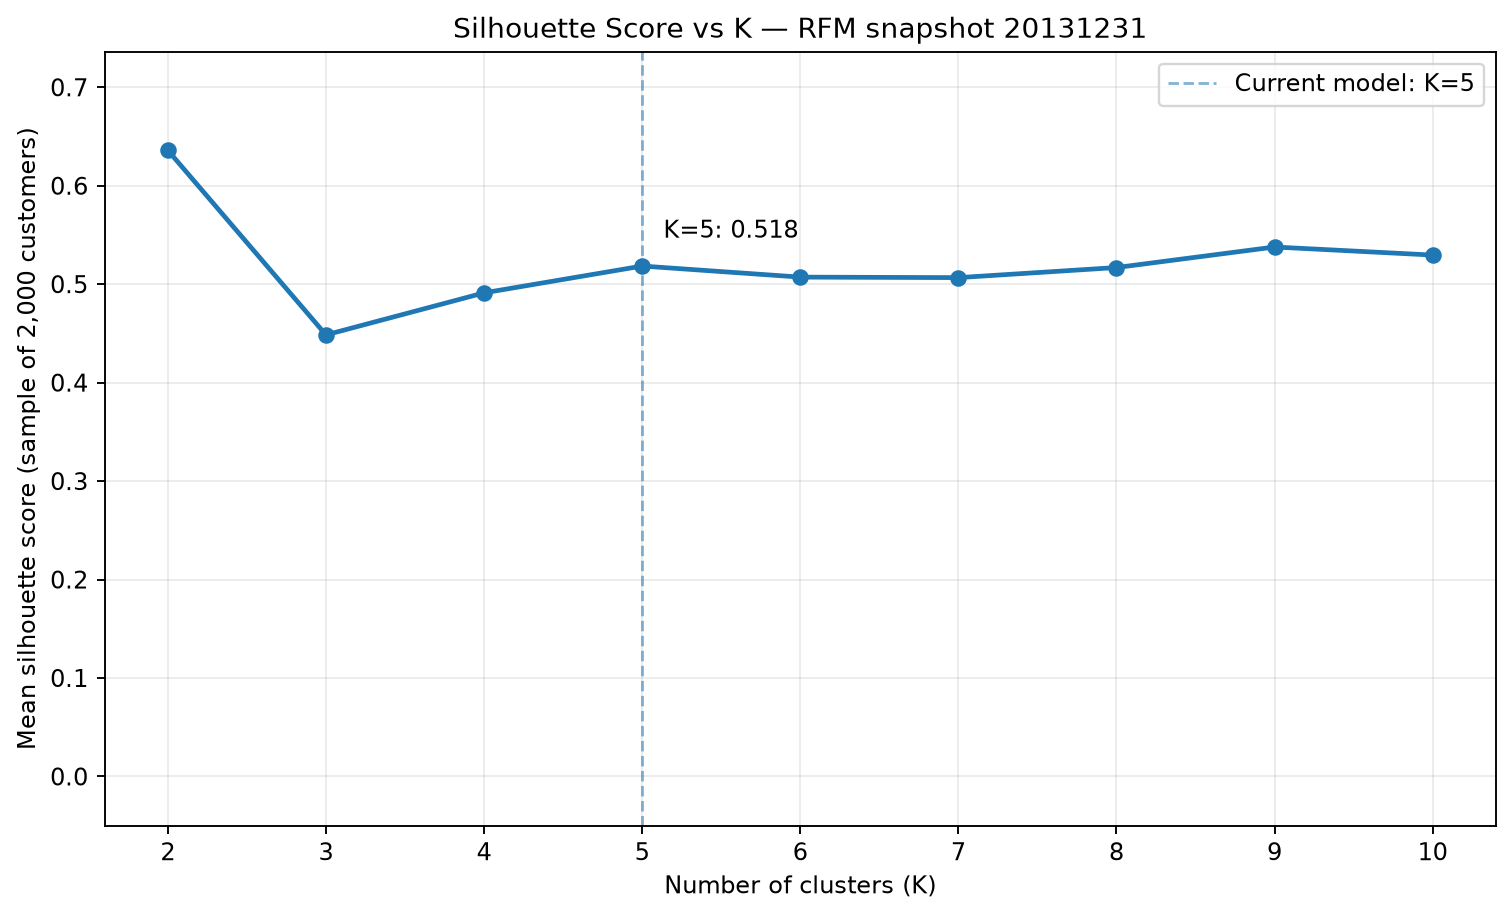
\includegraphics[width=0.94\textwidth]{silhouette_vs_k_20131231.png}
  \caption{Silhouette comparison for different cluster counts on the same snapshot.}
  \label{fig:silhouette_2013}
\end{figure}

K-Means only returns a numeric cluster ID (0 to 4) for each customer, which reflects no value of what the groups mean. Moreover,
annually the model is retrained and the number from 0 to 4 is different and not staying consistent. Therefore, to turn
them into meaningful clusters automatically, a solution is implemented: Each cluster on an RFM variable is given
``points'', based on how its average compares with the other clusters. The rules are

For Monetary and Frequency: the cluster with the highest average gets 5 points and the lowest get 1. (the higher these
values are, the more valuable they are)

For Recency: the rule is reversed because shorter time since the last purchase is better.

\noindent The implemented composite score is \(\text{Monetary rank}+\text{Frequency rank}+1.1\times\text{Recency rank}\).

Recency is weighted slightly higher, because a recent purchase is a strong sign that a customer is still active. Points
are given to clusters, not to individual customers.

The outcome will look like this:

\begin{table}[htbp]
  \centering
  \begingroup
  \scriptsize
  \setlength{\tabcolsep}{2pt}
  \begin{tabular}{rrrrrrrrl}
    \hline
    \textbf{Cluster} & \shortstack{\textbf{Avg}\\\textbf{Recency}} & \shortstack{\textbf{Avg}\\\textbf{Frequency}} & \shortstack{\textbf{Avg}\\\textbf{Monetary}} & \textbf{R points} & \textbf{F points} & \textbf{M points} & \textbf{Score} & \textbf{Segment}         \\
    \hline
    4                & 110.34                                      & 2.55                                          & 1,694.00                                     & 4                 & 5                 & 5                 & 14.4           & Champions                \\
    2                & 13.31                                       & 1.24                                          & 96.10                                        & 5                 & 4                 & 3                 & 12.5           & Recent / Promising       \\
    0                & 174.17                                      & 1.00                                          & 1,518.38                                     & 3                 & 2                 & 4                 & 9.3            & High-Value / Cooling Off \\
    3                & 196.03                                      & 1.03                                          & 48.91                                        & 2                 & 3                 & 2                 & 7.2            & Low-Spend / Occasional   \\
    1                & 602.92                                      & 0.00                                          & 0.00                                         & 1                 & 1                 & 1                 & 3.1            & Lost / Dormant           \\
    \hline
  \end{tabular}
  \endgroup
\end{table}

The example model output was recorded for an 18,484-customer analysis extract. The final dashboard chapter reports 18,485 customers for its June 2014 view. This one-record difference has not been reconciled in the submitted materials, so the two counts should not be presented as an identical population without verification.

Champions (cluster 4) has the highest frequency and spend, with an average of 2.55 purchases and 1,694 in total. Its
average recency is 110 days, so these customers are valuable but have not bought recently.

High-Value / Cooling Off (cluster 0) is the second-largest group by spend, but each customer has bought only once on
average. Their last purchase was about 174 days ago, so they are at risk of leaving.

Low-Spend / Occasional (cluster 3) is the largest group. Customers buy about once, spend about 49 on average, and last
bought about 196 days ago.

Recent / Promising (cluster 2) bought most recently, with an average of 13 days since the last purchase. Their spend is
low so far, which suggests they are new customers who may grow.

Lost / Dormant (cluster 1) has no recorded frequency or spend in the period, and an average recency of 603 days. These
customers have stopped buying.

\section{Conclusion}

The result of the RFM Analysis and K-Means clustering reveal the distinct customer segments with unique purchasing
behaviours. By standardizing the RFM variables and applying the K-Means algorithm, the dataset was successfully divided
into five interpretable clusters. Such segmentation highlights not only the diversity in customer engagement levels but
also provides valuable insights for strategic business decision-making. Therefore, the CompanyX will be able to design
and launch effective marketing strategies to each cluster of customers, not only to retain the occasional buyers, but
also to come up with attractive promotions for recent customers.

The first historical model was initialized with \texttt{bootstrap.py} from the 2011 year-end snapshot, including retrospective labels for earlier months. Separate 2012 and 2013 models were then saved with \texttt{train\_model.py}. The most recent active model is used by the Python live scorer. These saved model versions support repeatable clustering without retraining on every purchase.


% !TeX root = ../main.tex
\chapter{Business Intelligence \& Analytics Dashboards}
\label{chap:power_bi}

\section{Context \& Dashboard Objectives}
\label{sec:bi_context}

\subsection{Business Context}
\label{subsec:bi_business_context}
After completing the data warehouse and running the K-Means clustering model, our team needed an interactive tool to show the results to decision-makers. In the database, customer data and cluster numbers are stored in tables, which are difficult for managers to read and understand quickly. Therefore, we built a Business Intelligence (BI) dashboard using Microsoft Power BI.

The dashboard connects directly to the dimensional data warehouse and focuses on three main goals:
\begin{enumerate}
    \item \textbf{Executive Overview:} Help company directors monitor total sales, customer numbers, yearly trends, and early warnings about customer churn.
    \item \textbf{Customer Demographics:} Help marketing and sales teams understand customer profiles, such as location, income level, age group, gender, and job types.
    \item \textbf{RFM Segmentation and Strategy:} Help the CRM team see how each customer cluster behaves in terms of Recency, Frequency, and Monetary value, and choose the right marketing strategy for each group.
\end{enumerate}

\subsection{Visualization Principles from the Course}
\label{subsec:bi_principles}
To make sure the dashboard is easy to read and follows good data visualization rules, we applied the guidelines from \textcite{wilke2019fundamentals} and Dr. Phan Trong Nhan's lecture slides:
\begin{itemize}
    \item \textbf{Treemaps for Categories (Slide 31):} As taught in class, pie charts with more than 3 or 4 slices are difficult to read. We used treemaps to show customer occupation and segment breakdown clearly.
    \item \textbf{100\% Stacked Column Charts for Proportions over Time (Slide 50--51):} We used this chart type to compare how the percentage of each customer segment changed from 2011 to 2014.
    \item \textbf{Histograms for Distributions (Slide 54--55):} We grouped customer ages into clean bins ($<30$, $30-40$, $41-50$, $51-60$, $60+$) to show the age distribution of our buyers.
    \item \textbf{Bubble Chart for Multi-Variable Associations (Slide 57--59):} We plotted Recency on the X-axis, Monetary on the Y-axis, customer count as bubble size, and cluster colors to show the relationship between multiple metrics.
    \item \textbf{Consistent Colors across Pages (Slide 21):} We kept the exact same 5 colors for the 5 customer segments across all 3 pages so viewers do not get confused:
    \begin{itemize}
        \item \textcolor[rgb]{0.70, 0.13, 0.13}{\textbf{1. Champions:}} Red (\#A82020)
        \item \textcolor[rgb]{0.13, 0.35, 0.24}{\textbf{2. High-Value / Cooling Off:}} Dark Green (\#22593D)
        \item \textcolor[rgb]{0.85, 0.50, 0.10}{\textbf{3. Recent / Promising:}} Orange (\#D97F1A)
        \item \textcolor[rgb]{0.15, 0.60, 0.60}{\textbf{4. Low-Spend / Occasional:}} Teal (\#259696)
        \item \textcolor[rgb]{0.30, 0.15, 0.45}{\textbf{5. Lost / Dormant:}} Purple (\#4C2773)
    \end{itemize}
\end{itemize}

\subsection{Dashboard Structure}
\label{subsec:bi_hierarchy}
The report is organized into 3 main pages:
\begin{enumerate}
    \item \textbf{Page 1: Executive Customer \& Segmentation Overview} (High-level business health and trends).
    \item \textbf{Page 2: Customer Demographics \& Persona} (Detailed customer background information).
    \item \textbf{Page 3: Customer RFM Segmentation \& Behavior} (Detailed cluster metrics and strategic matrix).
\end{enumerate}

---

\section{Page 1: Executive Customer \& Segmentation Overview}
\label{sec:bi_page1}
Page 1 is designed for high-level managers who need a quick summary of the company's customer base, revenue, and retention status.

\begin{figure}[htbp]
    \centering
    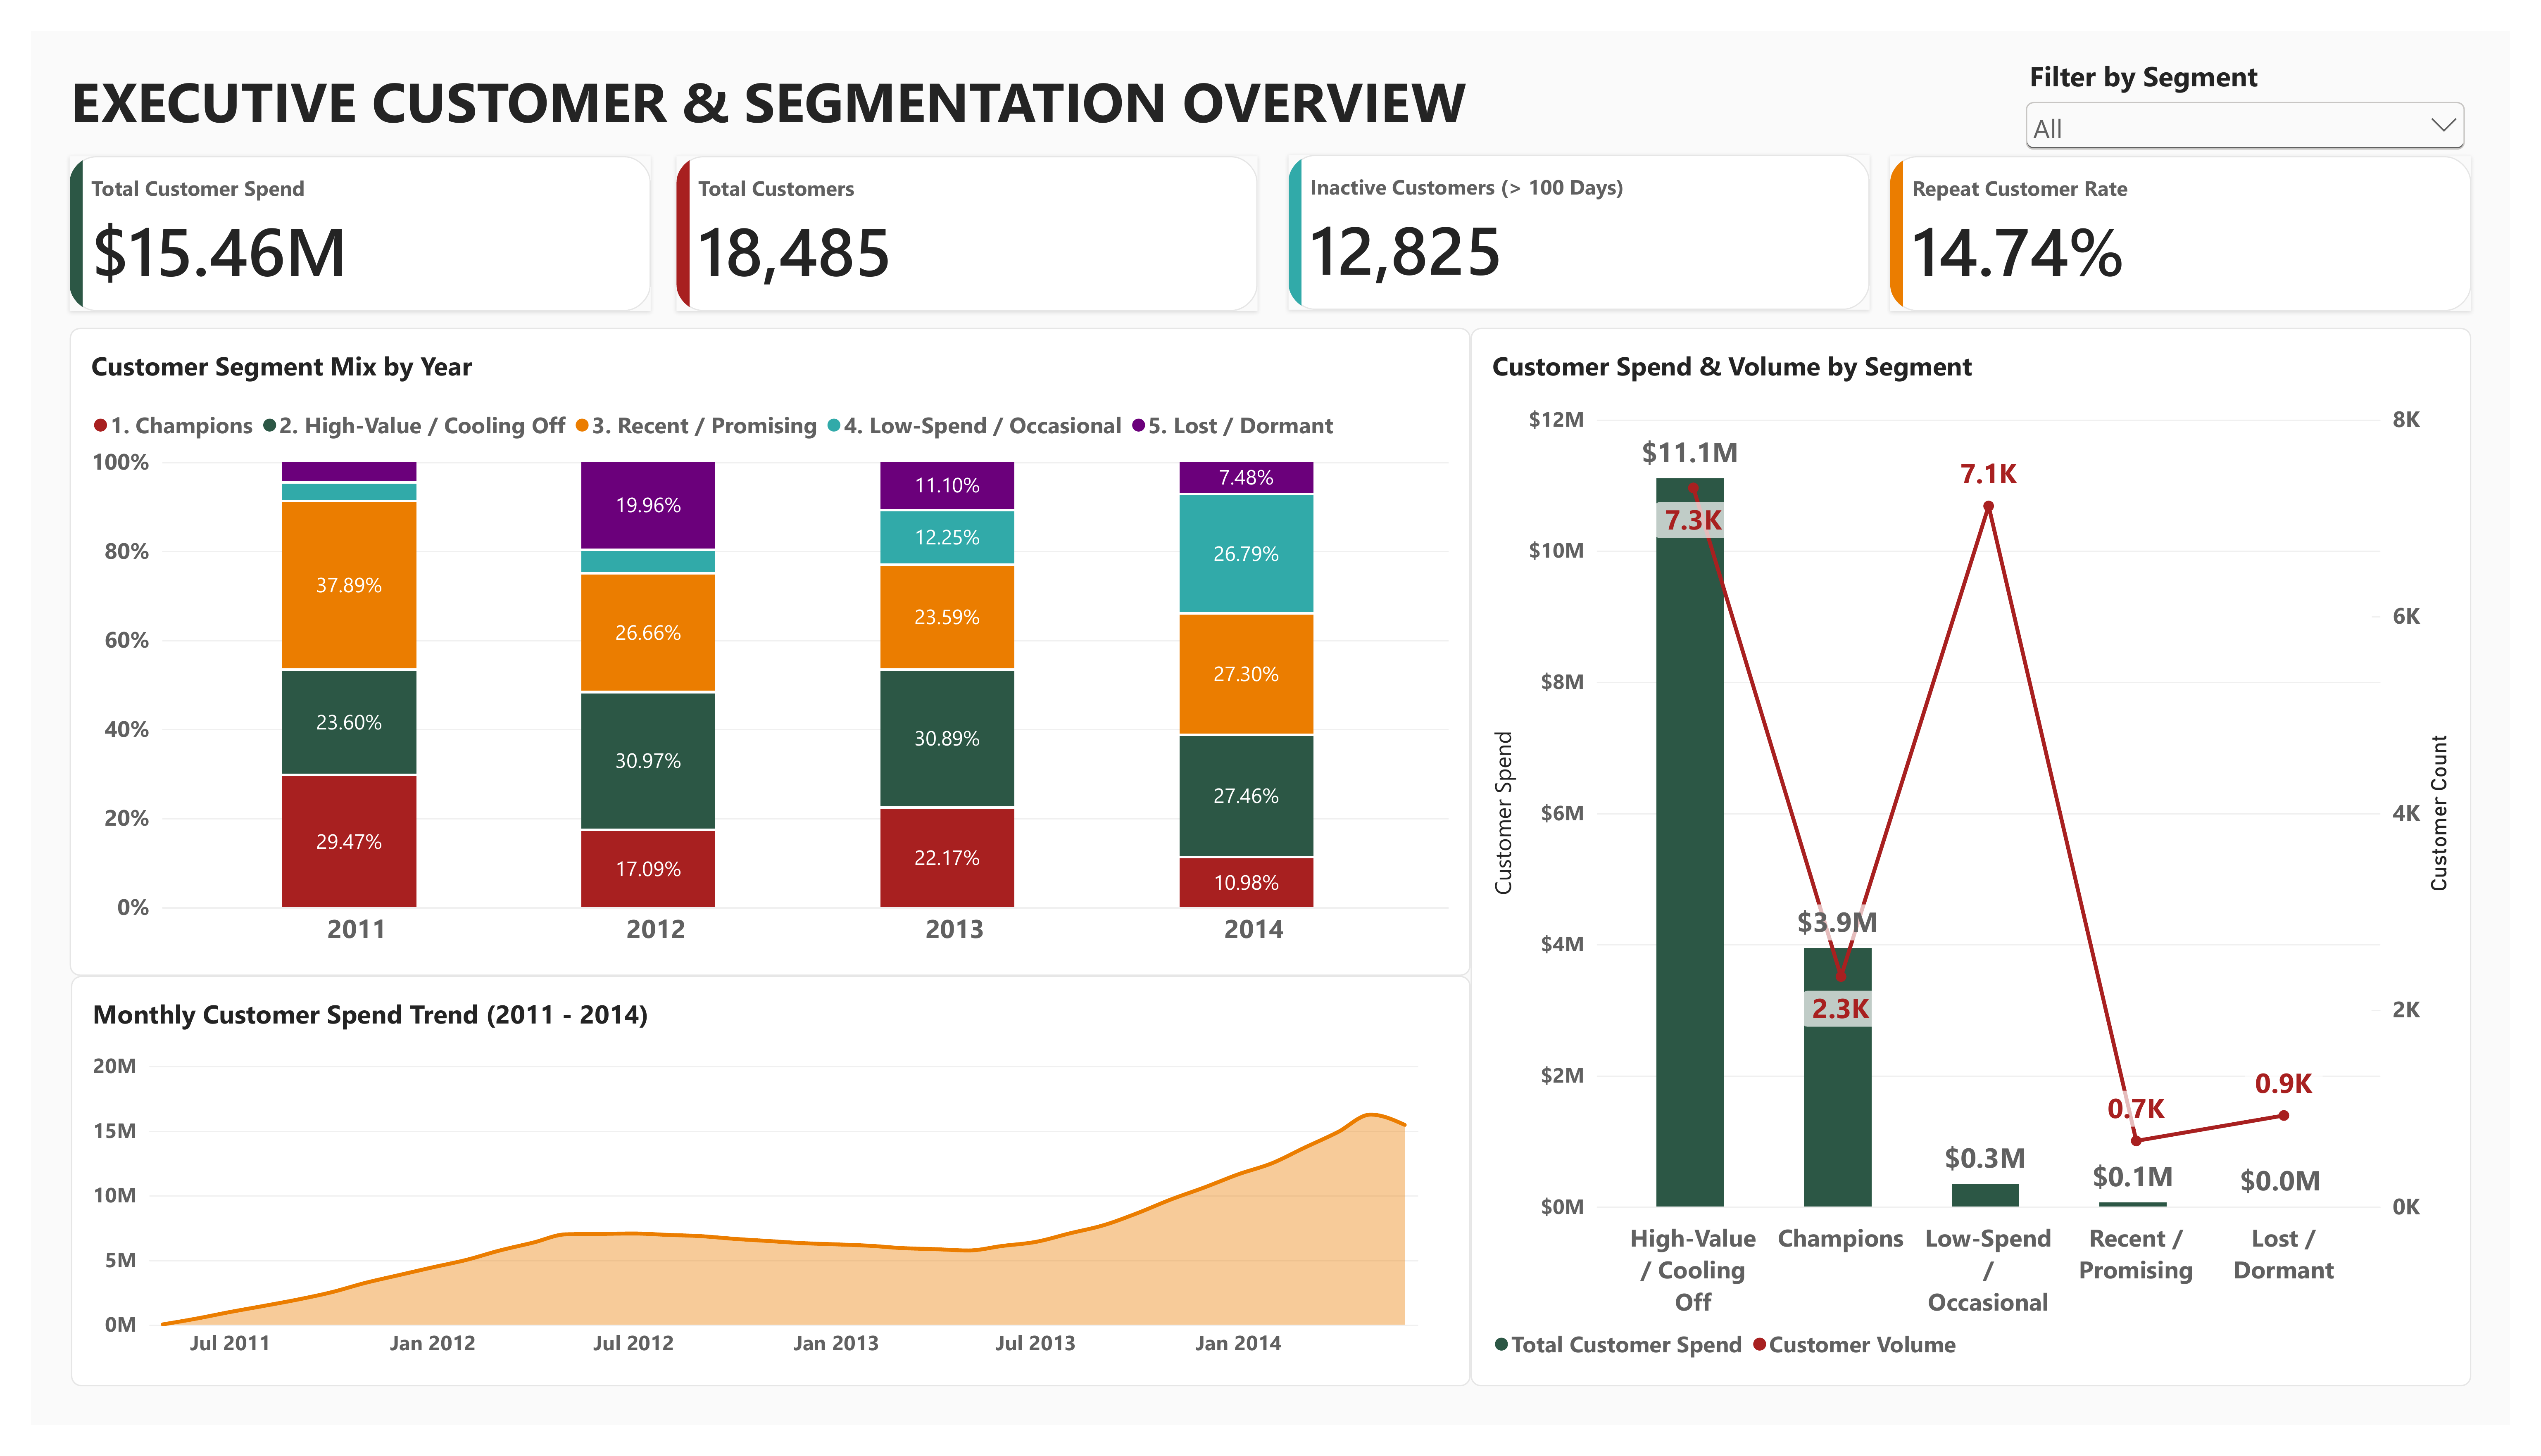
\includegraphics[width=\textwidth]{bi_page-1}
    \caption{Executive Customer \& Segmentation Overview Dashboard (Page 1).}
    \label{fig:bi_page1}
\end{figure}

\subsection{Core Executive KPIs}
\label{subsec:bi_page1_kpis}
At the top of Page 1, we place four key metrics:
\begin{enumerate}
    \item \textbf{Total Customer Spend (\$15.62M):} Total lifetime sales from all individual retail customers (\$15,615,354.05).
    \item \textbf{Total Customers (18,485):} Total number of unique customers in our database.
    \item \textbf{Inactive Customers ($> 100$ Days) (12,895):} The number of customers who have not made any purchases in the last 100 days. This makes up \textbf{69.76\%} of all customers. In the bicycle retail industry, bikes are durable goods, so people do not purchase every month. However, after 100 days (more than 3 months), if a buyer does not come back for small accessories or maintenance, they are at risk of leaving. Therefore, this KPI serves as an early-warning signal.
    \item \textbf{Repeat Customer Rate (14.96\%):} Calculated as the percentage of customers who have ordered at least two times:
    \begin{equation}
        \mathrm{Repeat\ Customer\ Rate} = \frac{\sum [ \mathrm{Customers\ with\ Frequency} \ge 2 ]}{\mathrm{Total\ Customers}} = \frac{2{,}765}{18{,}485} = 14.96\%
    \end{equation}
    This shows a serious business issue: \textbf{85.04\% of customers only bought once and never returned}.
\end{enumerate}

\subsection{Visual Charts and Key Findings}
\label{subsec:bi_page1_insights}
\subsubsection{1. Customer Segment Mix by Year (2011--2014)}
We selected a 100\% Stacked Column Chart to show the proportion of each customer segment over the four operational years:
\begin{itemize}
    \item \textbf{2011 Baseline:} In the first year, CompanyX focused on establishing its retail presence. \textit{Recent / Promising} customers constituted the largest group at \textbf{39.14\%}, followed by \textit{Champions} at \textbf{26.65\%} and \textit{High-Value / Cooling Off} at \textbf{24.49\%}. The \textit{Low-Spend / Occasional} and \textit{Lost / Dormant} segments formed only a small portion (roughly 9.7\% combined).
    \item \textbf{2012 Transition:} As earlier buyers matured, the proportion of \textit{High-Value / Cooling Off} customers increased to \textbf{31.57\%}. However, buyers who did not place repeat orders transitioned into \textit{Lost / Dormant}, which rose to \textbf{20.13\%}. The share of \textit{Champions} stood at \textbf{15.25\%}, while \textit{Recent / Promising} made up \textbf{27.02\%}.
    \item \textbf{2013 Product Diversification:} In 2013, the business began offering bike accessories and apparel. As a result, the \textit{Low-Spend / Occasional} segment grew substantially to \textbf{12.48\%}. The \textit{High-Value / Cooling Off} group remained steady at \textbf{31.39\%}, and \textit{Champions} accounted for \textbf{20.81\%}.
    \item \textbf{2014 Mass Market Expansion:} By 2014, the proportion of \textit{Low-Spend / Occasional} shoppers more than doubled to \textbf{26.78\%}. Meanwhile, \textit{High-Value / Cooling Off} represented \textbf{27.44\%}, \textit{Recent / Promising} was \textbf{27.34\%}, and \textit{Champions} made up \textbf{11.05\%}. The \textit{Lost / Dormant} group dropped to \textbf{7.39\%}.
\end{itemize}
These figures illustrate an important strategic shift: while CompanyX was originally a niche retailer of premium bicycles dominated by high-value buyers in 2011--2012, it successfully expanded to general everyday shoppers in 2013--2014. Nevertheless, this expansion brought a large volume of one-time or low-spending buyers.

\subsubsection{2. Monthly Customer Spend Trend (2011--2014)}
We used an Area Chart on a continuous date timeline from July 2011 to June 2014 to track overall revenue progression:
\begin{itemize}
    \item \textbf{Early Stage (2011--Mid 2012):} Monthly sales started at a moderate level, which was typical for a new business with a limited product catalog.
    \item \textbf{Rapid Acceleration (Mid 2012--End 2013):} Starting in the second half of 2012, sales increased significantly. The chart shows strong upward momentum throughout 2013, reaching the highest sales volume towards the end of 2013.
    \item \textbf{Seasonality Trends:} The area chart displays seasonal fluctuations, with higher sales during late spring and summer (peak outdoor cycling season) as well as year-end holiday shopping periods.
\end{itemize}

\subsubsection{3. Customer Spend \& Volume by Segment}
This Dual-Axis Combo Chart displays total sales as bars on the left axis and customer counts as points on the right axis:
\begin{itemize}
    \item \textbf{Validation of the Pareto Principle (80/20 Rule):}
    \begin{itemize}
        \item The \textit{High-Value / Cooling Off} cluster generates \textbf{\$11.2M} (71.53\% of total revenue) from 7,357 customers (39.80\% of the customer base).
        \item The \textit{Champions} cluster contributes \textbf{\$4.0M} (25.81\% of total revenue) from 2,377 customers (12.86\%).
        \item Together, these two premium segments contribute \textbf{97.34\%} of CompanyX's total lifetime sales (\$15.2M out of \$15.62M), while making up only \textbf{52.66\%} of all customers (9,734 people).
    \end{itemize}
    \item \textbf{The Low-Monetary Contrast:}
    In comparison, the \textit{Low-Spend / Occasional} group contains 7,175 customers (38.82\% of the total base) but brings in only \textbf{\$0.35M} (2.25\% of revenue). Similarly, \textit{Recent / Promising} accounts for \textbf{\$0.07M} (0.42\%), and \textit{Lost / Dormant} accounts for \textbf{\$0.00}.
    \item \textbf{Key Takeaway:}
    This clearly demonstrates that retaining high-value customers is far more essential for business survival than simply acquiring many low-spend shoppers.
\end{itemize}

\subsection{Dashboard Interactivity and Slicer Architecture}
\label{subsec:bi_page1_slicer_design}
In our Power BI solution, an interactive dropdown slicer (\textit{Filter by Segment}) is placed in the top-right corner of each dashboard page. However, during the dashboard development, an important architectural decision was required for Page 1:
\begin{itemize}
    \item \textbf{The Macro Trend Conflict:} The two longitudinal visuals---\textit{Customer Segment Mix by Year} and \textit{Monthly Customer Spend Trend}---rely on historical snapshot data from the periodic snapshot table (\texttt{FactCustomerSnapshot}) to show the whole company's evolution. In particular, the 100\% stacked column chart displays the structural proportions among all five segments. If a single segment is filtered, the multi-segment composition collapses to 100\%, eliminating its analytical purpose.
    \item \textbf{Implementation of Edit Interactions:} Following standard Business Intelligence best practices, we accessed the \textit{Format $\rightarrow$ Edit Interactions} menu in Power BI and set the interaction from the segment slicer to \textbf{None} for these two macro trend visuals. As a result, users can filter the top KPI cards and the segment combo chart without breaking the overall company baseline timeline.
\end{itemize}

---

\section{Page 2: Customer Demographics \& Persona Profiling}
\label{sec:bi_page2}
Page 2 helps us understand who our customers are, where they live, and what their personal characteristics look like.

\begin{figure}[htbp]
    \centering
    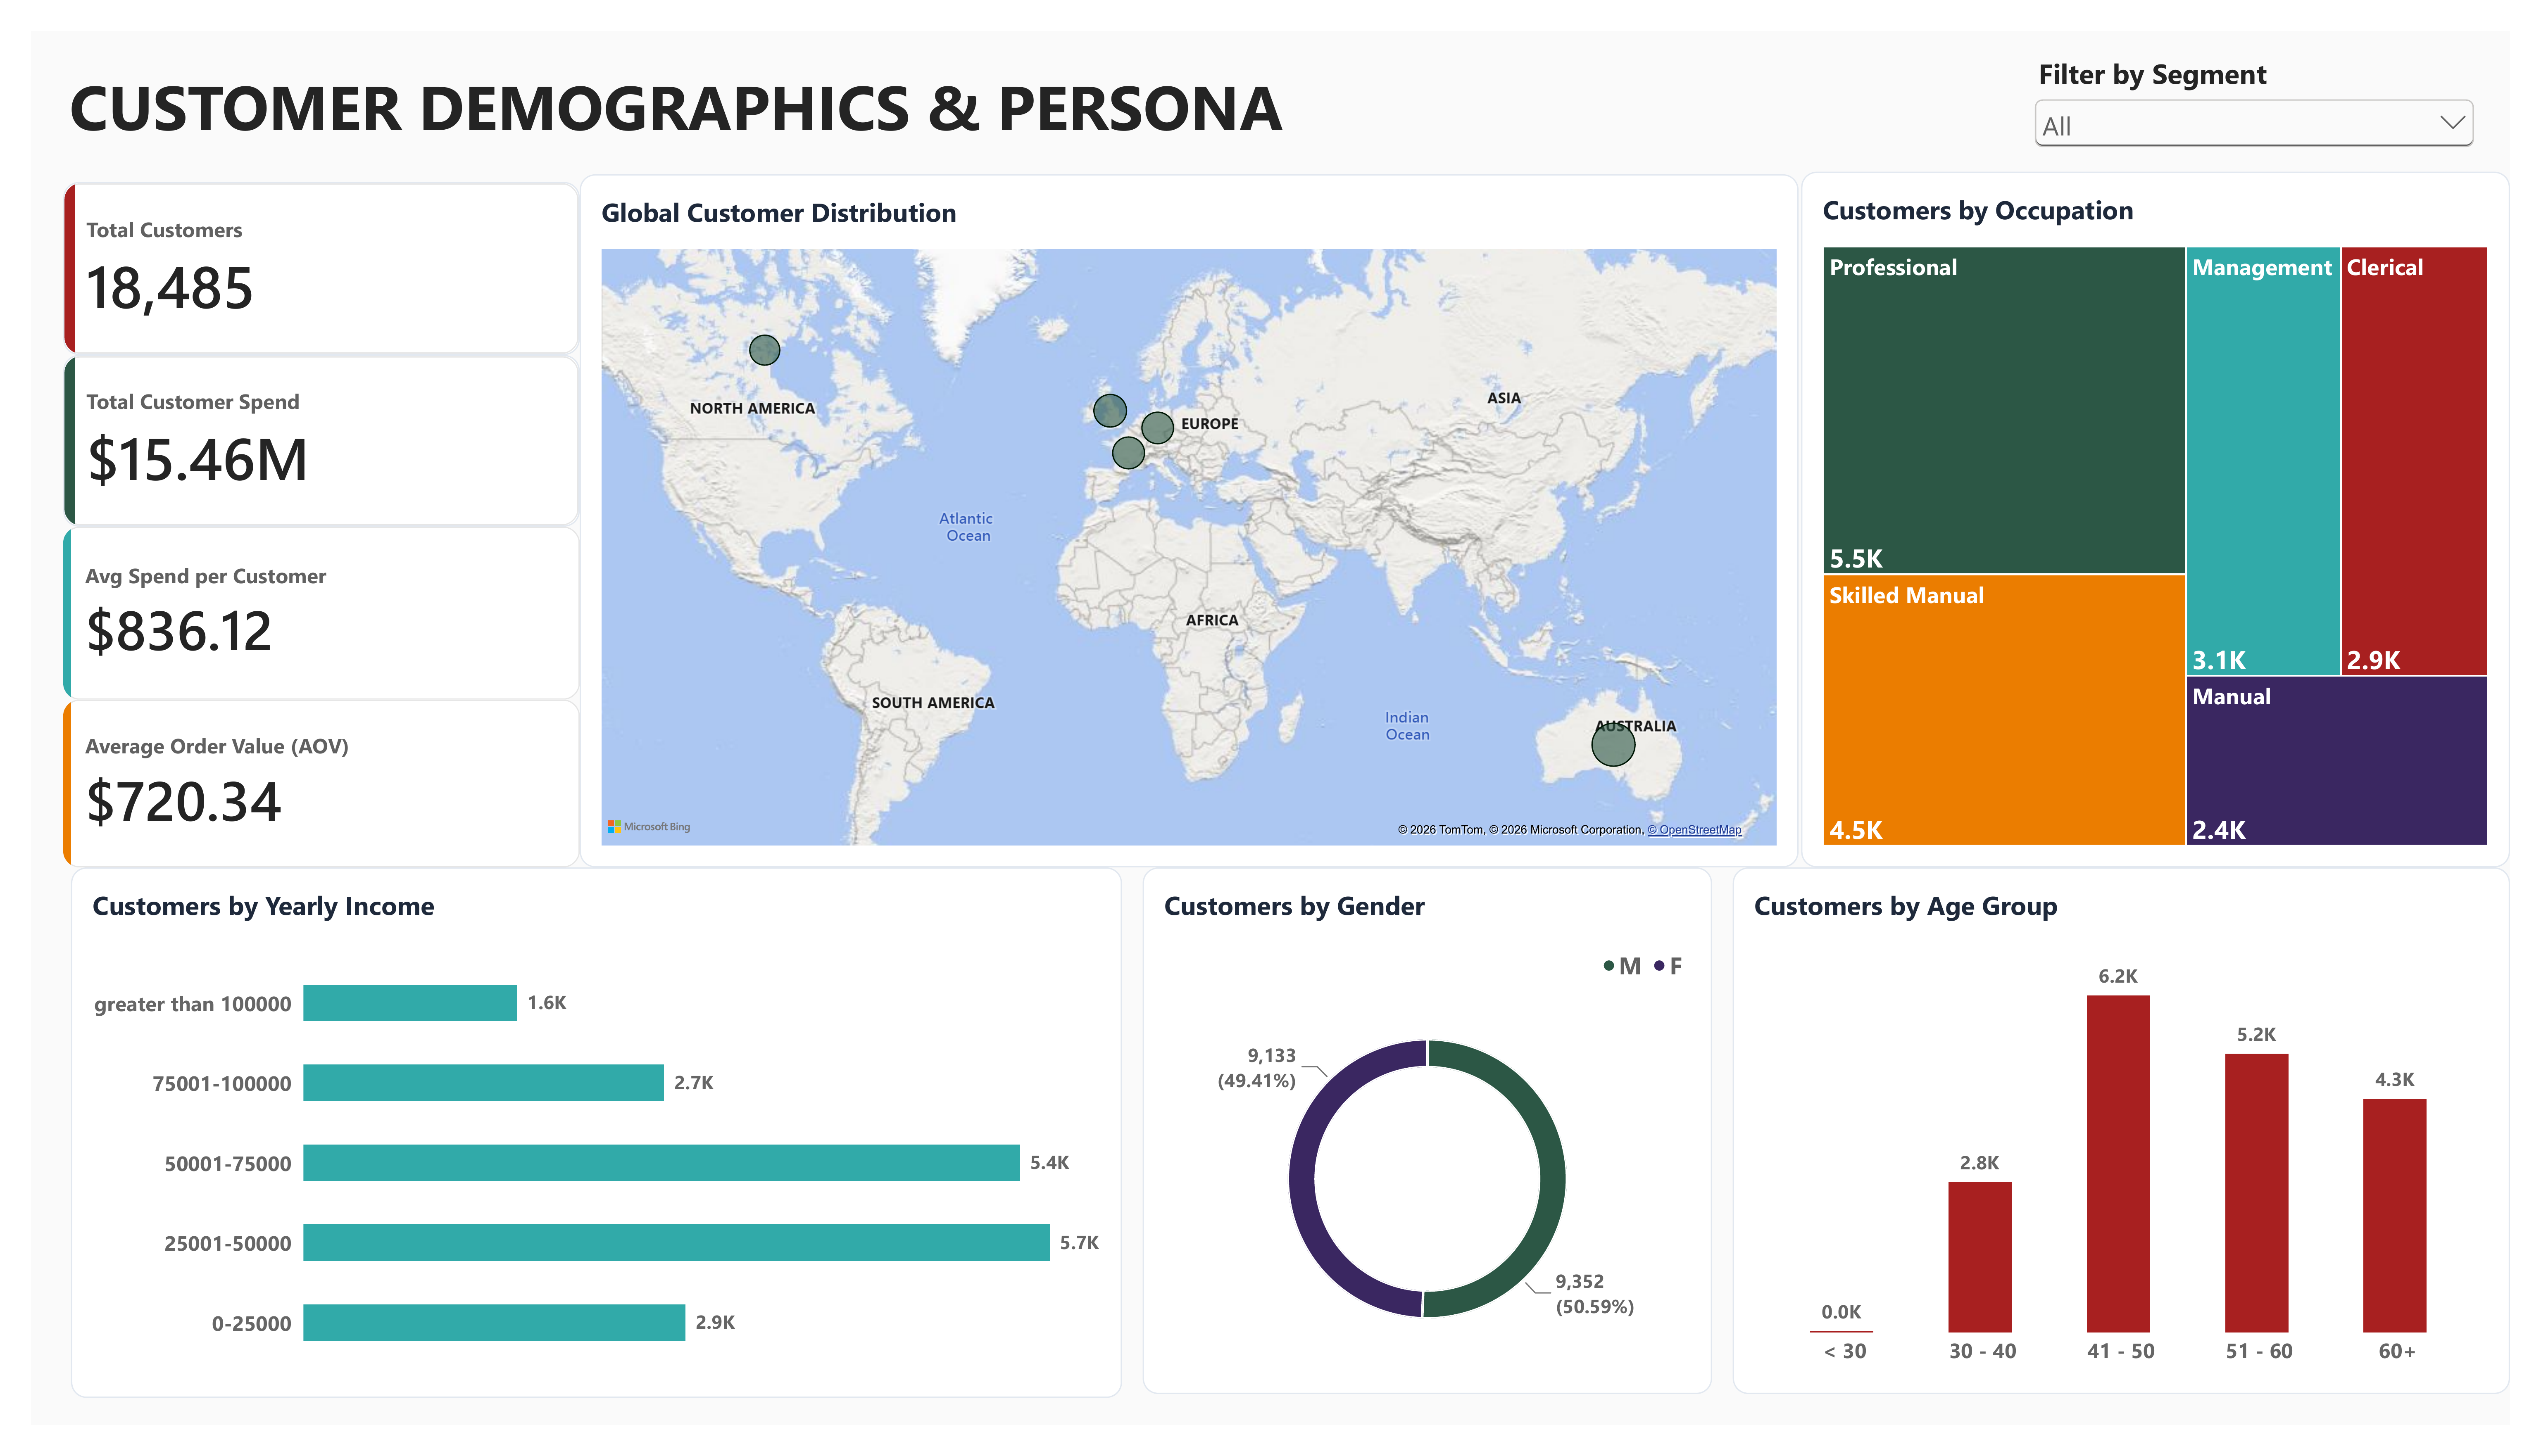
\includegraphics[width=\textwidth]{bi_page-2}
    \caption{Customer Demographics \& Persona Dashboard (Page 2).}
    \label{fig:bi_page2}
\end{figure}

\subsection{Demographic Overview KPIs}
\label{subsec:bi_page2_kpis}
The four cards on the left show customer averages:
\begin{itemize}
    \item \textbf{Total Customers:} 18,485.
    \item \textbf{Total Customer Spend:} \$15.62M.
    \item \textbf{Average Spend per Customer:} \textbf{\$844.76}.
    \item \textbf{Average Order Value (AOV):} \textbf{\$720.53}.
\end{itemize}
Because Average Spend (\$844.76) is very close to Average Order Value (\$720.53), it confirms again that most people only place one single order in their lifetime.

\subsection{Demographic Analysis (Overall Base)}
\label{subsec:bi_page2_insights}
\subsubsection{1. Geographic Distribution (Map Visual)}
The map shows that our customers live in developed markets with strong cycling cultures, mainly in North America (United States, Canada), Western Europe (United Kingdom, Germany, France), and Australia.

\subsubsection{2. Customers by Occupation (Treemap)}
\begin{itemize}
    \item \textbf{Professional} (5,505 people, 29.8\%) and \textbf{Skilled Manual} (4,577 people, 24.8\%) make up more than \textbf{54.6\%} of all customers.
    \item Other occupations include Management (3,075, 16.6\%), Clerical (2,928, 15.8\%), and Manual workers (2,400, 13.0\%).
    \item This shows that our core buyers are educated workers and skilled technicians who have good income and an active lifestyle.
\end{itemize}

\subsubsection{3. Customers by Yearly Income (Horizontal Bar Chart)}
\begin{itemize}
    \item The middle-income groups are the largest: \textbf{\$25,001--\$50,000} has 5,720 customers (30.9\%), and \textbf{\$50,001--\$75,000} has 5,496 customers (29.7\%).
    \item Together, middle-class customers make up \textbf{60.6\%} of the total customer base. High earners ($>\$100,000$) represent 1,600 customers (8.7\%), while entry-level earners (\$0--\$25,000) account for 2,870 customers (15.5\%).
\end{itemize}

\subsubsection{4. Customers by Gender (Donut Chart)}
\begin{itemize}
    \item \textbf{Male:} 9,352 customers (50.59\%).
    \item \textbf{Female:} 9,133 customers (49.41\%).
    \item The gender ratio is almost 50/50, which proves that cycling products are popular with both men and women equally.
\end{itemize}

\subsubsection{5. Customers by Age Group (Column Histogram)}
\begin{itemize}
    \item Customers are grouped into age brackets: $<30$, $30-40$, $41-50$, $51-60$, and $60+$.
    \item The majority of customers are in middle age: \textbf{41--50 years old} (6,200 people, 33.5\%) and \textbf{51--60 years old} (5,200 people, 28.1\%).
    \item People under 30 make up a very small portion, meaning that young adults rarely buy expensive bicycles from CompanyX.
\end{itemize}

\subsection{Segment-Specific Demographic Personas (Slicer Drill-Down)}
\label{subsec:bi_page2_personas}
By utilizing the interactive segment slicer on Page 2, decision-makers can drill down into the unique demographic persona of each customer cluster. Table~\ref{tab:segment_demographics} provides an empirical comparison across the five groups.

\begin{table}[htbp]
\centering
\caption{Comparative Demographic Profiles Across Customer Segments.}
\label{tab:segment_demographics}
\small
\resizebox{\textwidth}{!}{
\begin{tabular}{|l|r|r|r|l|l|l|}
\hline
\textbf{Segment} & \textbf{Customers} & \textbf{Total Spend} & \textbf{AOV (\$)} & \textbf{Top Occupation} & \textbf{Peak Income} & \textbf{Dominant Age} \\ \hline
1. Champions & 2,377 & \$4.03M & \$665.99 & Professional (39.2\%) & \$50k--\$75k (30.9\%) & 41--50 (38.3\%) \\ \hline
2. High-Value & 7,357 & \$11.17M & \$1,518.20 & Professional (29.9\%) & \$50k--\$75k (32.2\%) & 41--50 (39.4\%) \\ \hline
3. Recent & 679 & \$65.18K & \$77.22 & Skilled Manual (28.7\%) & \$25k--\$50k (29.8\%) & 60+ (29.5\%) \\ \hline
4. Low-Spend & 7,175 & \$350.92K & \$47.33 & Professional (27.9\%) & \$25k--\$50k (30.6\%) & 60+ (29.3\%) \\ \hline
5. Lost / Dormant & 897 & \$0.00 & \$0.00 & Skilled Manual (37.8\%) & \$25k--\$50k (43.5\%) & 41--50 (39.6\%) \\ \hline
\end{tabular}
}
\end{table}

\subsubsection{Key Findings from Segment Drill-Down}
Filtering each segment on Page 2 highlights significant differences in purchasing power, age distribution, and professional background:
\begin{enumerate}
    \item \textbf{1. Champions (Affluent White-Collar Repeat Buyers):}
    \begin{itemize}
        \item \textit{Highest Earning Power:} Champions have the highest income level among all clusters. Buyers earning more than \$100,000 account for \textbf{14.01\%} (333 individuals), while 30.88\% earn \$50,000--\$75,000.
        \item \textit{White-Collar Roles:} \textit{Professional} (39.17\%, 931 people) and \textit{Management} (18.93\%, 450 people) represent \textbf{58.10\%} of this group, demonstrating that corporate earners drive repeat purchases.
        \item \textit{Distinct Repeat Behavior:} This is the only segment where Average Spend per Customer (\$1,700) is much higher than Average Order Value (\$665.99). This confirms that Champions make multiple repeat transactions ($F \approx 2.55$), buying replacement parts and upgrades.
        \item \textit{Age Concentration:} Heavily centered in the \textbf{41--50} age bracket (\textbf{38.33\%}, 911 buyers), followed by 51--60 (27.93\%). These are established professionals investing in active health and cycling hobbies.
    \end{itemize}

    \item \textbf{2. High-Value / Cooling Off (Single-Purchase Premium Buyers):}
    \begin{itemize}
        \item \textit{Spend Equals AOV:} Average Spend per Customer exactly equals Average Order Value at \textbf{\$1,518.20}. This proves that these 7,357 customers purchased one high-end bicycle and have not yet returned.
        \item \textit{Solid Middle Class:} The largest income groups are \$50,001--\$75,000 (32.17\%) and \$25,001--\$50,000 (31.58\%), representing \textbf{63.75\%} of the cluster.
        \item \textit{Age Group:} The dominant bracket is 41--50 years old (39.42\%, 2.9K buyers), followed by 51--60 (28.55\%, 2.1K buyers).
    \end{itemize}

    \item \textbf{3. Recent / Promising (Older Entrants \& Skilled Technicians):}
    \begin{itemize}
        \item \textit{Unexpected Age Shift:} In contrast to Champions and High-Value clusters, the single largest age group in \textit{Recent / Promising} is \textbf{60+ years old} (\textbf{29.46\%}, 200 customers). This demonstrates that senior riders and retirees represent a growing acquisition channel.
        \item \textit{Occupation Distribution:} \textit{Skilled Manual} (28.72\%, 195 people) surpasses \textit{Professional} (27.54\%, 187 people) as the leading occupation.
        \item \textit{Early Repeat Signals:} With an AOV of \$77.22 and an average spend of \$95.99, a subset of customers have already completed second accessory orders within two weeks ($R = 13.28$ days).
    \end{itemize}

    \item \textbf{4. Low-Spend / Occasional (Budget-Conscious Accessory Shoppers):}
    \begin{itemize}
        \item \textit{Lower-Income Skew:} This group contains the highest percentage of lower-income shoppers: buyers earning below \$25,000 account for \textbf{20.60\%} (1,478 individuals).
        \item \textit{Job Breakdown:} \textit{Manual} workers represent 16.7\% (1.2K people, tied with Management), which is the highest manual laborer proportion among all active clusters.
        \item \textit{Age Profile:} Like the Recent segment, this cluster has a heavy concentration of seniors aged \textbf{60+} (\textbf{29.3\%}, 2.1K buyers), alongside a noticeable group of younger adults aged 30--40 (18.1\%).
        \item \textit{Basket Size:} The AOV is very small at \textbf{\$47.33}, confirming that these customers only buy minor accessories such as inner tubes, water bottles, and helmets.
    \end{itemize}

    \item \textbf{5. Lost / Dormant (Disengaged Lower-Income Manual Workers):}
    \begin{itemize}
        \item \textit{Occupation Disparity:} \textit{Skilled Manual} workers heavily dominate at \textbf{37.79\%} (339 buyers), while \textit{Management} drops to its lowest proportion at \textbf{8.70\%}.
        \item \textit{Compressed Earnings:} Over \textbf{80.49\%} of customers earn between \$25,000 and \$75,000, with only 4.24\% earning above \$100,000.
        \item \textit{Complete Inactivity:} With \$0.00 in spend and over 600 days without an order, these contacts have churned from the brand.
    \end{itemize}
\end{enumerate}

---

\section{Page 3: Customer RFM Segmentation \& Behavioral Matrix}
\label{sec:bi_page3}
Page 3 explains the 5 customer clusters from our K-Means model using the RFM framework (Recency, Frequency, Monetary).

\begin{figure}[htbp]
    \centering
    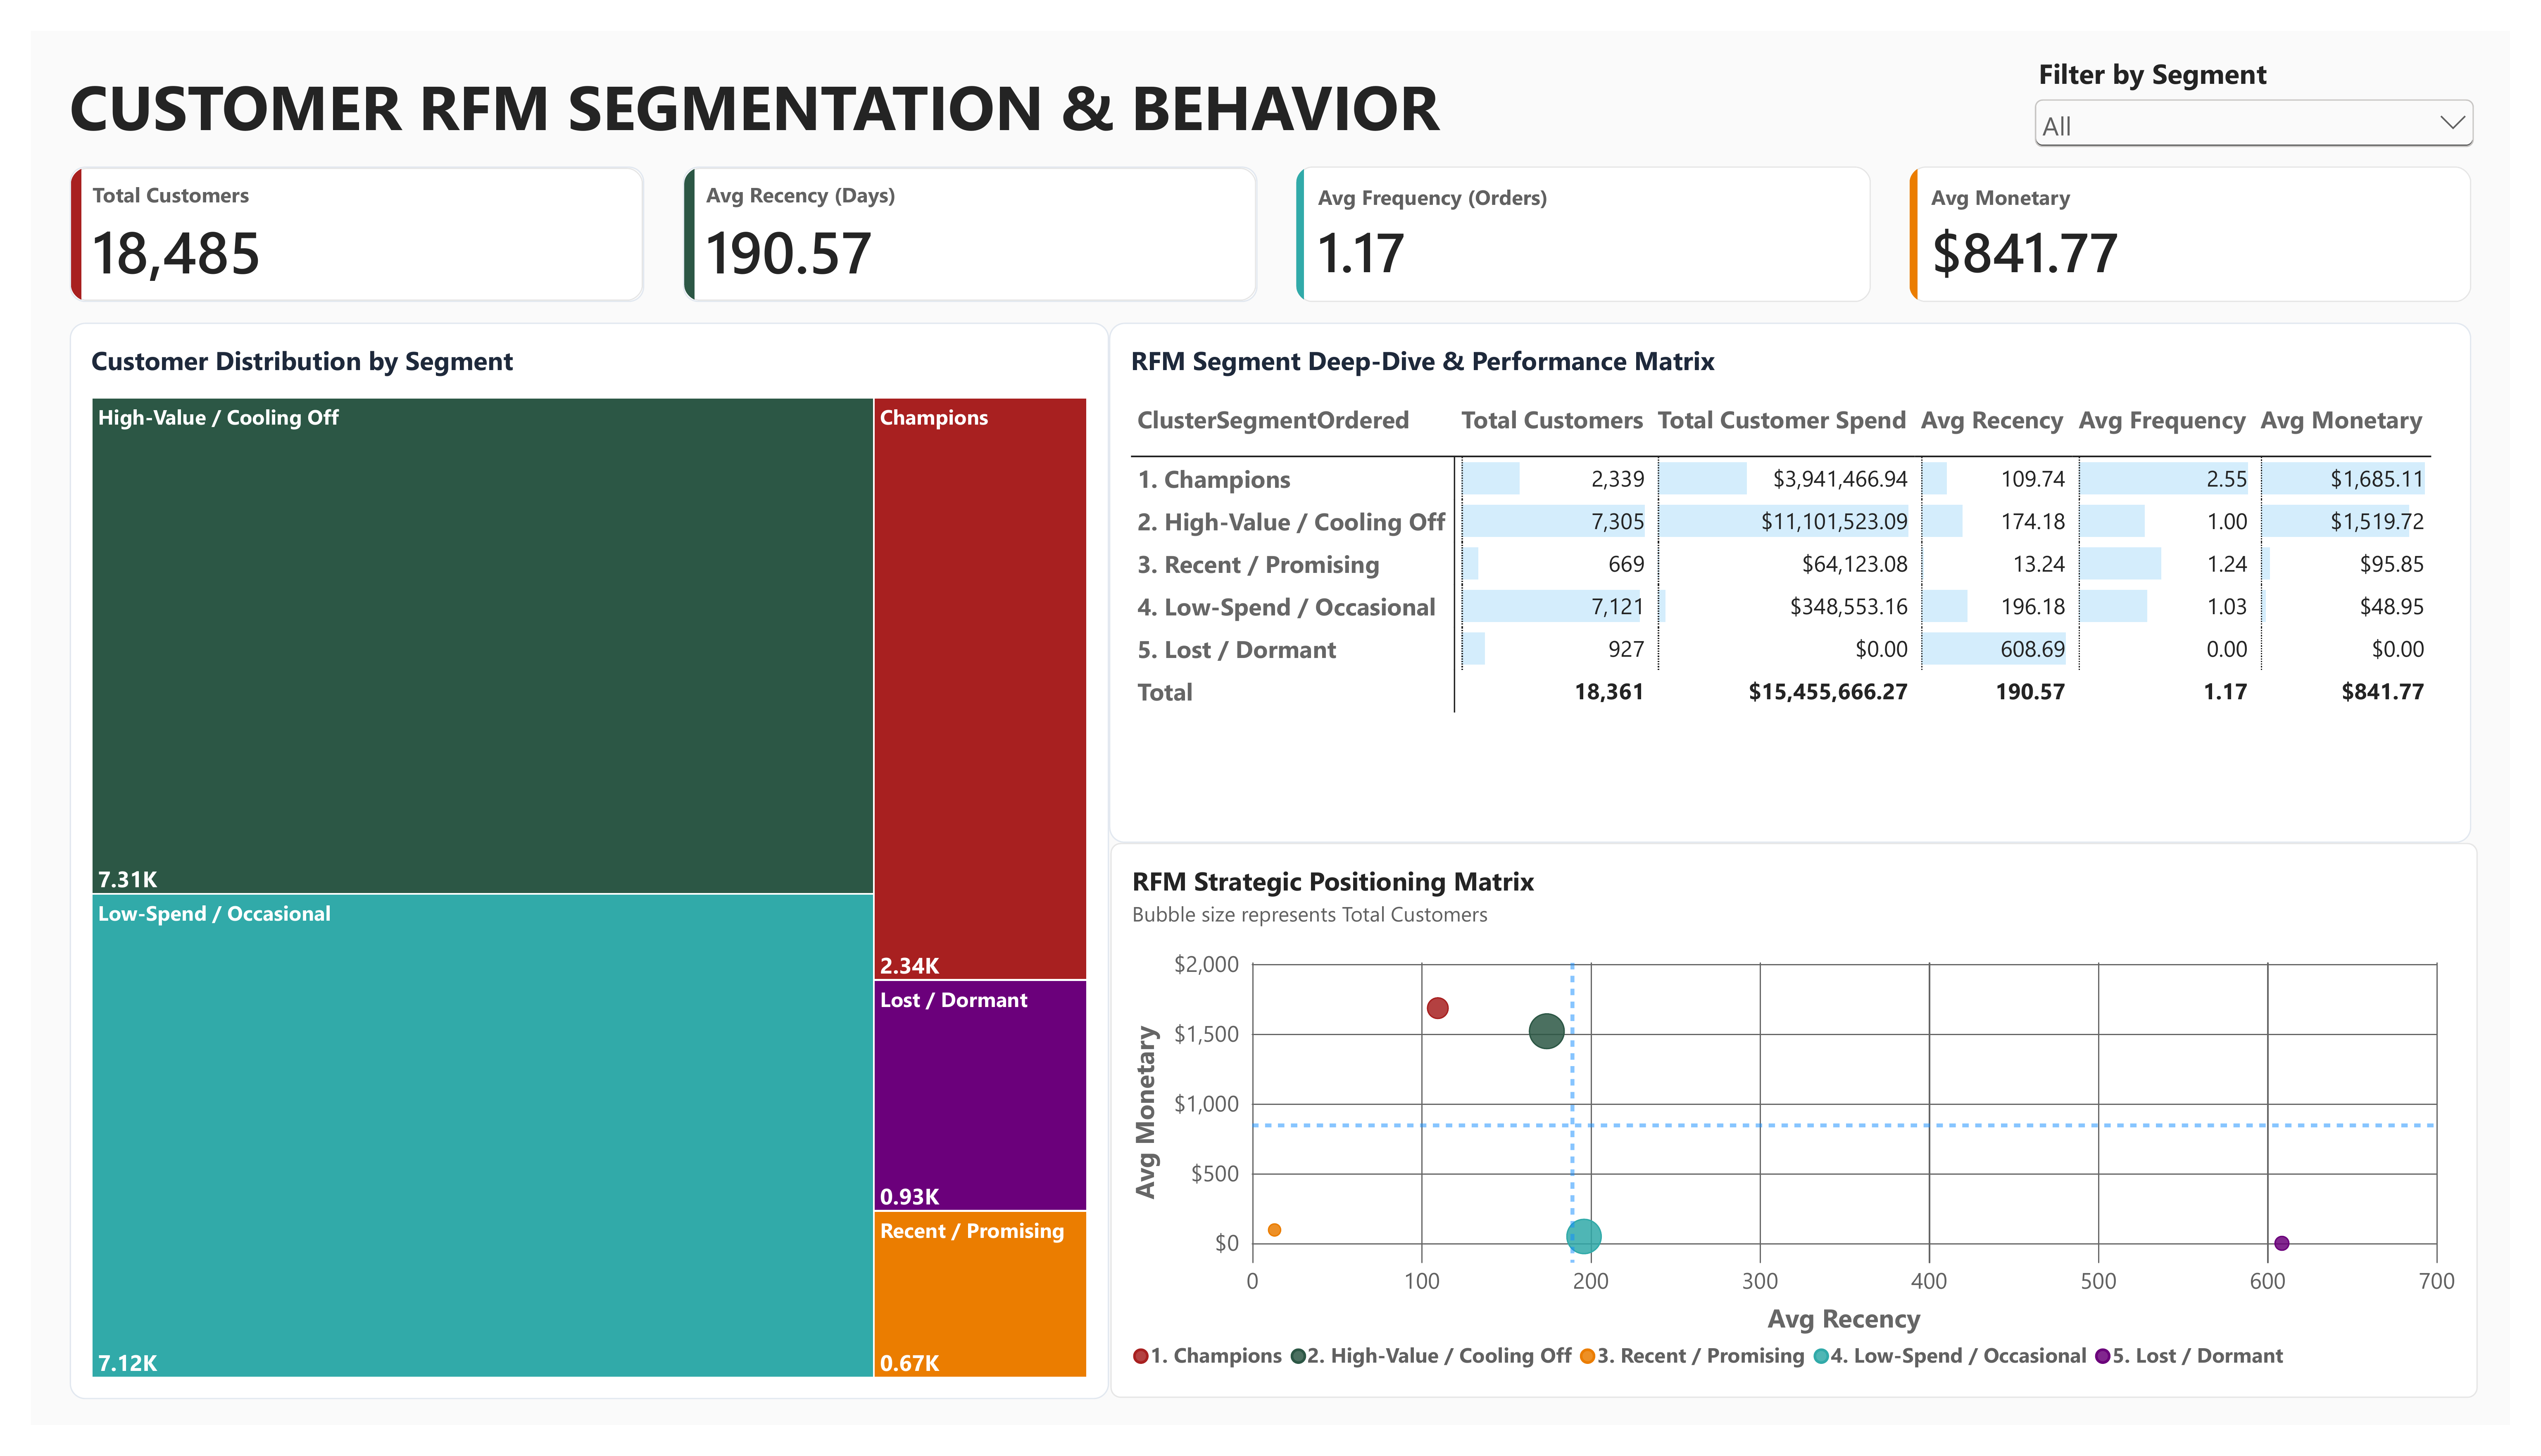
\includegraphics[width=\textwidth]{bi_page-3}
    \caption{Customer RFM Segmentation \& Behavior Dashboard (Page 3).}
    \label{fig:bi_page3}
\end{figure}

\subsection{Company-Wide Benchmark Metrics}
\label{subsec:bi_page3_benchmarks}
The top ribbon gives the overall company averages:
\begin{itemize}
    \item \textbf{Average Recency:} \textbf{189.32 Days} (around 6.3 months since the last order).
    \item \textbf{Average Frequency:} \textbf{1.17 Orders} per customer.
    \item \textbf{Average Monetary:} \textbf{\$844.76} total spend per customer.
\end{itemize}

\subsection{Cluster Performance Table}
\label{subsec:bi_page3_matrix}
Table~\ref{tab:rfm_matrix} shows the exact statistics for each of the 5 segments:

\begin{table}[htbp]
\centering
\caption{Customer RFM Cluster Statistics.}
\label{tab:rfm_matrix}
\small
\setlength{\tabcolsep}{4.5pt}
\begin{tabular}{|l|r|r|r|r|r|}
\hline
\textbf{Cluster Segment} & \textbf{Customers} & \textbf{Total Spend (\$)} & \textbf{Avg R (Days)} & \textbf{Avg F} & \textbf{Avg M (\$)} \\ \hline
1. Champions & 2,377 (12.86\%) & \$4,029,883.62 & 110.17 & 2.55 & \$1,695.37 \\ \hline
2. High-Value / Cooling Off & 7,357 (39.80\%) & \$11,169,375.36 & 174.19 & 1.00 & \$1,518.20 \\ \hline
3. Recent / Promising & 679 (3.67\%) & \$65,175.19 & 13.28 & 1.24 & \$95.99 \\ \hline
4. Low-Spend / Occasional & 7,175 (38.82\%) & \$350,919.88 & 196.01 & 1.03 & \$48.91 \\ \hline
5. Lost / Dormant & 897 (4.85\%) & \$0.00 & 602.92 & 0.00 & \$0.00 \\ \hline
\textbf{Company Total / Average} & \textbf{18,485} & \textbf{\$15,615,354.05} & \textbf{189.32} & \textbf{1.17} & \textbf{\$844.76} \\ \hline
\end{tabular}
\end{table}

\subsection{Customer Volume Distribution (Donut Chart)}
\label{subsec:bi_page3_donut}
The donut chart on the left side of Page 3 illustrates the relative share of each customer group:
\begin{itemize}
    \item \textbf{High-Value / Cooling Off:} 7,357 customers (\textbf{39.80\%} of total volume).
    \item \textbf{Low-Spend / Occasional:} 7,175 customers (\textbf{38.82\%}).
    \item \textbf{Champions:} 2,377 customers (\textbf{12.86\%}).
    \item \textbf{Lost / Dormant:} 897 customers (\textbf{4.85\%}).
    \item \textbf{Recent / Promising:} 679 customers (\textbf{3.67\%}).
\end{itemize}
This chart emphasizes that more than 78\% of the customer base is divided almost evenly between two contrasting groups: high-spending buyers who need urgent retention, and low-spending buyers who make infrequent accessory purchases.

\subsection{Strategic Positioning Matrix (Bubble Chart)}
\label{subsec:bi_page3_positioning}
The bubble chart at the bottom-right plots all 5 clusters:
\begin{itemize}
    \item \textbf{X-Axis:} Average Recency (from 0 to 700 days). Lower is better.
    \item \textbf{Y-Axis:} Average Monetary (from \$0 to \$2,000). Higher is better.
    \item \textbf{Bubble Size:} Total number of customers in the cluster.
    \item \textbf{Benchmark Lines:} Dotted reference lines at company averages ($X = 189.32$ days and $Y = \$844.76$) divide the chart into four quadrants.
\end{itemize}

\subsubsection{Quadrant Analysis}
\begin{enumerate}
    \item \textbf{Top-Left (High Spend, Low Recency) --- Champions:}
    These customers bought recently ($R=110.17$ days) and spend the most ($M=\$1,695.37$). They are our best VIP customers.
    \item \textbf{Top-Center (High Spend, Moderate Recency) --- High-Value / Cooling Off:}
    These customers spent a lot ($M=\$1,518.20$), but their Recency is 174.19 days, which is close to the 189-day average. They are starting to cool down and need immediate attention before they leave.
    \item \textbf{Bottom-Left (Low Spend, Very Recent) --- Recent / Promising:}
    These are new customers who bought recently ($R=13.28$ days). Their spend is still small (\$95.99), but they have great potential to grow into Champions.
    \item \textbf{Bottom-Right (Low Spend, High Recency) --- Low-Spend \& Lost:}
    These customers have not bought for a long time and spend very little. The Lost group has not returned for over 600 days.
\end{enumerate}

---

\section{Actionable Business Recommendations}
\label{sec:bi_recommendations}
Based on the dashboard insights, we recommend the following practical strategies for CompanyX:

\subsection{1. Champions: VIP Loyalty Program}
\label{subsec:rec_champions}
\begin{itemize}
    \item \textbf{Goal:} Keep our best customers happy and encourage them to recommend the brand to others.
    \item \textbf{Action:} Create a VIP club that gives early access to new bicycle models, invitations to special cycling events, and referral discounts when they introduce friends.
\end{itemize}

\subsection{2. High-Value / Cooling Off: Urgent Retention Campaigns}
\label{subsec:rec_high_value}
\begin{itemize}
    \item \textbf{Goal:} Protect the most important revenue source (over 71\% of total sales).
    \item \textbf{Action:} Set up an automated email at day 120 after their purchase offering a free annual bicycle check-up at local partner shops, or a \$150 discount voucher if they upgrade components within 30 days.
\end{itemize}

\subsection{3. Recent / Promising: Cross-Selling and Welcome Series}
\label{subsec:rec_recent}
\begin{itemize}
    \item \textbf{Goal:} Encourage new buyers to make a second purchase quickly.
    \item \textbf{Action:} Send a 30-day email series: Day 3 with bike assembly and safety tips, Day 14 with cleaning advice, and Day 21 offering a 15\% discount on essential accessories like helmets, gloves, and lights.
\end{itemize}

\subsection{4. Low-Spend / Occasional: Low-Cost Automated Marketing}
\label{subsec:rec_low_spend}
\begin{itemize}
    \item \textbf{Goal:} Increase purchase frequency without spending too much marketing budget.
    \item \textbf{Action:} Avoid expensive phone calls or printed mail. Instead, send automated emails and seasonal clearance announcements for cheap consumables like water bottles and spare tubes.
\end{itemize}

\subsection{5. Lost / Dormant: Cost Reduction}
\label{subsec:rec_lost}
\begin{itemize}
    \item \textbf{Goal:} Stop wasting advertising money on inactive contacts ($R > 600$ days).
    \item \textbf{Action:} Remove this group from paid Facebook and Google ads. Only send them one or two broad holiday sale emails per year (e.g., Black Friday or New Year).
\end{itemize}

---

\section{Summary of Core DAX Measures}
\label{sec:bi_dax_summary}
Table~\ref{tab:dax_summary} summarizes the main DAX formulas created in Power BI for this project:

\begin{table}[htbp]
\centering
\caption{Summary of Core DAX Measures.}
\label{tab:dax_summary}
\small
\begin{tabular}{|l|l|p{7.5cm}|}
\hline
\textbf{Measure Name} & \textbf{Home Table} & \textbf{DAX Formula / Logic} \\ \hline
Total Customers & FactCustomerRFMLive & \texttt{DISTINCTCOUNT(CustomerKey)} \\ \hline
Total Customer Spend & FactCustomerRFMLive & \texttt{SUM(Monetary)} \\ \hline
Inactive Customers (>100d) & FactCustomerRFMLive & \texttt{CALCULATE([Total Customers],} \newline \texttt{\phantom{X}Recency > 100)} \\ \hline
Repeat Customer Rate & FactCustomerRFMLive & \texttt{VAR R = CALCULATE([Total Customers],} \newline \texttt{\phantom{XXXXXX}Frequency >= 2)} \newline \texttt{RETURN DIVIDE(R, [Total Customers], 0)} \\ \hline
Average Order Value (AOV) & FactCustomerRFMLive & \texttt{DIVIDE([Total Customer Spend],} \newline \texttt{\phantom{XXXXXXX}SUM(Frequency), 0)} \\ \hline
Avg Spend per Customer & FactCustomerRFMLive & \texttt{DIVIDE([Total Customer Spend],} \newline \texttt{\phantom{XXXXXXX}[Total Customers], 0)} \\ \hline
Monthly Customer Spend & FactCustomerSnapshot & \texttt{SUM(MonetarySnapshot)} \\ \hline
\end{tabular}
\end{table}


\newpage
% UPDATED: Command to output the bibliography
\printbibliography

\end{document}